% !Mode:: "TeX:UTF-8"

\chapter[并行计算简介]{并行计算简介}
\section{并行计算产生的背景}

在社会需求和技术更新迭代的推动和促进下,高性能计算成为许许多多应用应用领域的必须。
许多应用领域,如生物计算,卫星云图计算,基因对比,经济金融计算,股票交易等等领域对计算能力需求已越来越高,这
大规模的大数据量计算需要刺激和激发了大规模并行计算的流行和兴起,对并行计算提出了更多的要求
,但是曾经还缺乏标准的支持,出现并行计算标准混乱的情况。其实,并行是终必将在所有计算机中展现出来—
—包括个人数字助理、PC计算机、工作站,计算集群及超级计算机等。

计算机的出现深刻了影响了现代科技,世界经济发展,文化生活,出现在人类生活学习工作的各个脚步,
计算机的迅猛发展也带动了其他学科的快速发展。随着网络技术、计算机科学,计算机理论的快速发展
计算机对经济与科技生活的影响日益深入,刺激和引发了更多的计算需求,反过来促进和推动了高性能计
算技术。现代自然科学甚至社会科学参与的各领域,如:计算流体力学、 计算结构力学、生物医学、人工智能及模式识别、
量子化学、核磁共振、油藏模拟、密码破译等,已经出现了高性能计算的需求。

1992年初,美国高性能计算与通信计划(HPCC)提出了在科学与工程计算领域中对国民经济与国
家安全都具有深远影响的一些重大挑战性课题,其中包括全球气候变化、长期天气预报、海洋环流建模、
湍流分析、空气动力学、三维生物结构、三维等离子体研究、四维时空结构、催化剂设计、药物分子结构设计、结
构生物学、人体基因与遗传工程、数字剖析、图像理解等方面。没一个课题都适合使用并行计算处理,同时
没一个重大课题无不涉及到了极大额计算量,无一不对计算机性能提出了高要求。

传统的单机技术能力较弱,与大量的计算数据需求执行形成了极大的矛盾,形成新的并行计算标准势在必行
计算机必将走向并行发展的道路,海量数据的计算需求必将成为推动并行机体系结构不断向前发展和演进的原超级力。

并行计算与并行算法是计算数学和新一代的计算机结合的产物,为了能够在尽量短的时间实现大量
大型数值计算问题的,不仅仅需要功能完善的并星际,还需要合理的,能够在并行机上应用的合理的并行算法

并行计算给了解决打计算量问题的新的思路,并行计算功能强大,性能强大,规模强大,具有巨大的
数值计算和数据处理能力,能够对社会带来巨大的经济效益.

    
并行计算的研究目的主要是将复杂问题并行分解为可被多个小部分解决的子问题,后将这些小问题分配
由多个计算机结点以进行并行处理,最后汇集各个计算结点的计算结果最后综合起来以得到最终结果。
总而言之,并行计算是为了加快运算速度和解决大主存容量的求解问题,
而发展起来的多计算机/多处理机的并行编程技术。

并行处理技术的诞生和进一步的发展,正是相应了时代的召唤,适应了大数据量的计算需求,尤其是在当今
云计算的背景下。

\section{并行计算发展}
\subsection{并行计算发展历程}
并行处理技术的发展先后经历了几个阶段:

60年代中期,先后产生了以鲍勒斯公司的ILLAC-IV为代表的单指令流多数据流的阵列处理机和以
CDC公司的STAR-100、CRAY公司的CRAY-1为代表的单处理机多流水线向量机。同时,我国也诞生了YH-1巨型机。
微程序控制的计算机开始普及。为了减小CPU和主存储器之间的速度差距,计算机采用了流水线和高速缓存;
同时为了使CPU和I/O操作在支持多用户程序和多任务管理,开始提供多程序的支持。

70年代开始,出现了用分布存储器、共享存储器和向量硬件选件的不同结构并行计算机,用于并行计算处理
的多处理操作系统开始发展,多处理器编程序言和相应的多语言编译器开始出现。出现了用于并行处理或
分布式计算的软件工具和环境,SMP方式的总线协议,出现了共享主存的并行多处理系统(SPP机)。这
段时期的代表系统:CrayX-MP,IBM/3090VF,VAX9000,BBNTC-2000等。SPP类型的YH-2和曙光-I机型也开始
出现。并行处理技术在70年代开始逐渐成熟发展。

1972,超级计算机ILLIAC-IV的诞生,标志这大规模并行处理机(MPP)的兴起,其本身更成为并行处理的模范样本。
二以CRAY为代表的向量机由于天然良好的可编程性,仍然占据主机市场。 
80年代后期,向量机的造价成本上升,然而性能的提高却无法随着造价的提高而直线提高,导致向量机被迅速淘汰
,MPP从而成为主流的并行计算技术。MPP系统采用具有可伸缩性和可容时延性的系统结构,采用了VLSI硅片、砷
化嫁技术、高密度组装,光技术等先进技术。Fujitsu的VPP500,Cray Research的MPP,Cray公司的T3D,Th
inking Machines公司的CM-5和Intel超级计算机系统Paragon即是MPP系统的代表。

\textbf{???}目前,新一代的并行计算系统正在加紧研制之中,除了单个节点的处理性能更高外,节点之间互连所采用的方式和结构也是讨论的热点话题。由基于NUMA(Non-Uniform Memory Access)方式构成的分布共享存储器组成的并行机系统,特别是采用目录方法来保持各Cache之间数据一致性的CC-NUMA(Cache Coherent NUMA),由于其具有良好的可伸缩性和可编程性,将是未来高端超级计算机的一个重要发展方向。另外随着快速以太网、超高速吠太网和ATM网络的不断普及和性能的不断提高,由高性能微机或工作站组成的计算机机群进行并行处理的各种技术也成为了当前研究的焦点课题。
\subsection{并行计算发展现状}
    并行计算的研究目前主要集中在理论研究,应用研究和并行程序设计三方面.在理论研究方面,
主要是研究并行程序的描述,体系结构,设计与实现并行算法,负载均衡等方面.
    
    在并行计算的应用研究方面,正在努力让并行算法实现良好的可移植性,形成一次编译,到处运行
的优势,设计出稳定高效的硬件设备,通信设备;解决和降低执行并行程序时处理器之间的相互通讯问题,
,减小和优化通信开销

    在并行程序设计方面,主要研究如何运用现有的编程语言和软件环境,分解原串行程序的问题,
分治到多个计算结点上,以满足大规模并行应用的需要.

    归结并行计算机的发展历史以及应用现状,目前的并行计算机系统主要有以下四类:
\begin{enumerate}
\item 多向量处理系统,如Fujitsu VP-2000和NEC SX-3等;

\item 基于共享存储的多处理机系统(SMP/Shared Memory multiProcessors ,SPP/Shared memory Parallel multiProcessors),
如SGI Power Challenge、曙光1号等;

\item 基于分布存储的大规模并行处理(MPP)系统,如Intel Paragon、IBM SP2、曙光1000等;

\item 基于RISC工作站或大量服务器借助高速互连网络连接而成的机群计算机系统(Cluster),如清华同方探索集群计算机、曙光天潮机群等。
\end{enumerate}

通过上述四类主流并行机及相关并行技术的发展态势可以得到一下结论:并行软件和并行算法的发展远远落后于并
行计算机系统的发展。并行和分布式计算应用的发展远远落后于并行和分布式计算技术的发展。综上所述:
\begin{enumerate}
\item 并行计算正在朝软件硬件一体化的方向来构成并行和分布计算系统平台发展。
\item 并行计算机系统的可伸缩性和可编程性已成为限制并行计算进一步发展,并成为主要瓶颈。
\item 主要研究领域不再是大规模并行处理机系统。由于负载平衡难于实现,并且相应的并行算法设计困难,
据国外专家预测,MPP在高性能计算机市场即所占的份额将快速降低
\item 基于分布共享存储器(Distributed Shared Memory, DSM)结构的并行机系统, 具有良好的可伸缩
性和可编程性,已受到诸多计算机厂商的青睐,各类并行机系统已经存在市场之中
\item 由高速网络互联而成的可伸缩的计算机机群系统,由于具有超高的性价比和有效性而发展很快,加
上可移植异构编程环境PVM(Parallel Virtual Machine)和标准的消息传送平台MPI(Message Passing Interface)的a
进一步成熟和应用,极大地反馈和刺激了并行计算的发展.
\end{enumerate}

\subsection{国内外并行计算发展现状}
并行计算机具有功能多、性能高、规模大的特点,具有巨大的数值计算和数据处理能力,能够广泛应用于国民经济、
国防建设、科技发展等个项领域中。随着计算机和算法的发展,在科学发展的各个领域都向定量化和精确化发展,由此而导致对计算速度的不断增长,例如在石油勘探、地震预测预报、气候模拟及大范围天气预报、新型武器设计和核武器系统的研究模拟、地质研究、天体和地球科学、虚拟现实系统等等都需要大量的计算来解决。要解决这些问题,用传统的串行算法很难解决,必须要使用并行计算。并行计算给了我们一个解决大计算量的一般方法。使用并行计算机可以解决这些在一般计算机上难以解决的问题,具有巨大的社会和经济效益。在国际上,高科技竞争日益激烈,而并行计算技术已成为体现一个国家综合实力的一种标志,它
对保障国家安全、促进科技进步、推动经济发展有着不可替代的重要作用。 对高速并行计算的需求是广泛的,主要集中在三种类型的的应用需求:计算密集型,如数值模拟;数据密集型,如数据仓库;网络密集型,如远程医疗等。
而正是这些重大的应用领域推动了计算技术的发展。

1993年,美国科学、工程、技术联邦协调理事会向国会提交了题为“重大挑战项目:高性能计算和通讯(High Performance Computing and Communications Program)”的报告,简称 HPCC 计划。它列出了支持科学模拟、先进计算机辅助设计和大型数据库玉信息检索操作的实时处理等所需要的处理速度和存储器容量的量级。美国在高性能计算机的研究中一直处于领先状态,IBM 正在研制的名为“ASCI Purple”的超级计算机,计算速度比目前世界上最快的计算机、日本NEC 的地球模拟器(计算速度为每秒 35 万亿次浮点运算)快 3 倍。美国购买这台超级计算机,主要是用它来模拟发生核爆炸情景下对周围环境及人类的影响。另外一台名为“蓝色基因”的超级计算机,被美国称为“紫计划”,速度是每秒 360 万亿次浮点运算,比地球模拟器快 10 倍。主要用非军事研究,比如生命科学中基因、蛋白质的研究,或者石油勘探、车船制造中模拟车子的碰撞来提高车子的性能。这台名为“ASCI Purple”的超级计算机,计算速度比目前世界上最快的计算机、日本 NEC 的地球模拟器(计算速度为每秒 35 万亿次浮点运算)快 3 倍。美国购买这台超级计算机,主要是用它来模拟发生核爆炸情景下对周围环境及人类的影响。另外一台名为“蓝色基因”的超级计算机,被美国称为“紫计划”,速度是每秒360 万亿次浮点运算,比地球模拟器快 10 倍。主要用非军事研究,比如生命科学中基因、蛋白质的研究,或者石油勘探、车船制造中模拟车子的碰撞来提高车子的性能。

我国计算机技术起步较晚,而且西方国家奉行高性能技术不出口政策,在高性能计算机方面对我国实行严格禁运
措施,加上计算机教育起步的落后,总体导致了我国现在的并行计算机技术相对落后。而且,对与高性能计算机要
用的CPU,我国自我制造的龙芯性能还不够出众,但已经使我国在研制完全自主知识产权的高性能计算机方面有了
新的希望。最近几年,我国高性能计算机的开发和研制取得了长足的进展,自主研制开发和制造了系列曙光高性能计
算机,使我国成为世界上少数能够开发和生产高性能计算机的国家之一。

我国的并行计算机技术与美国等计算机发达国家相比,存在着一定的差距。发达国家的科技企业、国防
部门和高水平的科学研究部门,如MIT,哈佛医学院等等都在使用高性能并行计算。而我国高性能计算的应
用还未得到应用部门的普遍重视,但并行计算已经开始在气象等部门开始使用,随着我国政府加大对
超级计算机研制的支持力度,。同时,不但要发展硬件技术,同时,算法本身也是关键技术,如何让并行计算机实现最高的性能,则依赖算法的具体实现。

    

\section{并行计算平台}
    并行计算需要系统软件方面的支撑,常见的并行计算平台使用的大部分操作系统都采用了开源免费的Linux操作系统

\subsection{并行计算软件-Linux操作系统}
    Linux操作系统是一种自由和开放的操作系统,其目标是类Unix.Linux操作系统原为Linux内核,由Linus Torvalds在1991年10月5号发布.
本身linux仅仅代表Linux内核,在包含进更多的GUI组件和其他许多使用工具后,成为完整的Linux操作系统

    Linux被移植到了很多计算机硬件平台,具有优秀的可移植性.Linux同时作为一个领先的操作系统,
可以运行在服务器或者其他大型平台上,如大型主机和超级计算机.世界上的TOP500超级计算机采用
的都是Linux发行版.同时Linux系统也被移植到广大的嵌入式系统上,很多电视机盒,手机操作系统等等
都采用的是Linux操作系统.

    Linux操作系统采用的GNU通用公共许可证,任何人和机构都可以自由地使用Linux的所有底层源代码
,也可以自由地修改和再发布.1993年Richard Stallman发起GNU计划,制造出了c编译器,GNU C库和基本的命令行使用程序
.Linus Torvalds 和Richard Stallman合作推出了Linux,形成了一套完整的操作系统,自由软件基金会提议
将组合系统命名为GNU/Linux,包含了大量的GNU软件,包括一个Shell程序,必要的libc函数库,c/c++
编译器和工具等等. 现在,在Linus Torvalds的领导下,全世界众多的开发者都在共同参与开发Linux内核,而richard 
Stallman领导的自由软件基金会则继续提供大量的可以在Linux内核上使用的,

    Linux具有设备独立性,内核具有强大的适应力,能够给系统提供更高的可靠性.Linux发行版一直在被用来做
服务器的操作系统,并且独占奥头,许多云服务器公司都在使用Linux操作系统作为其基础软件部分的
一部分,其也经常做为超级计算机和并行计算机群的操作系统.
    
    Linux系统的特点:
    \begin{itemize}
    \item 开放性:Linux系统遵循国际POSIX标准,可以在遵循此标准的软件和硬件上使用,实现兼容,
方便的互连,同时Linux操作系统是开放内核源代码的,方便各种用户和商业用户进行改革
    \item 多用户:系统资源可以被不同的用户各自使用,每个用户对自己的资源,如文件,设备等等
进行控制,拥有自己的用户空间
    \item 多任务:计算机可以同时执行多个程序,程序之间不会相互影响.Linux采用抢占调度的多任务方式
,用户可以充分利用计算机软硬件资源
    \item 先进的网络功能,Linux是较早支持TCP/IP协议的操作系统之一,在网络通信方面优于其他
操作系统,内涵文件传输协议和远程访问
    \item 可靠的安全性:Linux内涵了多种安全技术措施,包括对用户的读,写权限控制,内核空间和
用户空间的分离,各用户之间的隔离,提供了许多必要的安全保障
    \item 良好的移植性: 能够从微机,嵌入式版本到大型计算机的任何环境和平台上运行,为不同的计算机平台
与其他机器进行准确,有效的通信提供了手段.
    \end{itemize}
\subsection{并行计算-程序设计}
    目前,并行程序设计常用3重并行程序编程环境,可以分为三类:消息传递,共享存储,数据并行,x
下表为各个并行编程环境的简单介绍

    \begin{table}[htbp]
    \centering  % 表居中
    \begin{tabular}{lccc}  % {lccc} 表示各列元素对齐方式,left-l,right-r,center-c
    \hline
    特征&消息传递&共享存储&数据并行\\ \hline 
    典型特征&MPI,PVM&OpenMP&HPF\\        
    可移植性&所有流行并行机&SMP,DSM&SMP,DSM,MPP\\      
    并行粒度&进程级大粒度&线程级大粒度&进程级细粒度\\     
    并行操作方式&异步&异步&松散同步\\   
    数据存储模式&分布式存储&共享存储&共享存储\\
    数据分配方式&显示&隐式&半隐式\\
    入门难度&较难&容易&简单 \\
    扩展性&好&较差&一般\\ \hline
    \end{tabular}
    \caption{三种并行编程环境的主要特征}
    \end{table}

\subsection{并行计算机-硬件分类}
    并行计算机的的硬件实现环境即并行计算环境,是直接影响并行计算赖以生存的基础,根据据名的
Flynn分类法,根据指令流与数据流的特点进行区别.指令是指执行的指令流;数据流是指指令调用的
数据流,如I/O流,即输入输出数据.可以把计算机系统分类成一下分类
    \begin{enumerate}
    \item 单指令流多数据流SISD
    \item 单指令流单数据流SIMD
    \item 多指令流多数据流MISD
    \item 多指令流单数据流MIMD
    \end{enumerate}
\subsubsection{SISD}
    SISD计算机是传统的单进程计算机,指令顺序执行,单次执行一条指令,并且只对单个数据流进行处理
\subsubsection{SIMD}
    向量处理机是典型的SIMD并行机.向量机利用流水线的概念,将计算机的指令执行拆分开,分为多段,
每个流水线的不同时间段处理不同的数据流,通过时间上的重叠实现效率叠加.向量处理机在并行计算机的
发展历史上起到了推动的作用,由于后期性价比不高,加之处理器性能的不断增强,向量处理机推出了历史
舞台
\subsubsection{共享存储的MIMD并行机}
    共享存储MIMD并行多处理机,通过高速互联网络共享一个统一的内存空间,通过内存数据实现处理机
之间的协调.对于各个计算结点,每个计算节点可以执行不同的执行程序或者相同的执行程序,但是数据流
不同,以实现不同的数据处理和计算任务.各个结点的通信可以通过共享存储实现,这种结构方便并行程序的
编写,执行效率高.但是当结算节点较多时,当处理器太多时,会加重内存的竞争,这时可以通过告诉缓冲
高速缓冲技术等来实现数据的高速交换.
\subsubsection{分布存储的MIMD并行机}
    由于共享存储的MIMD并行机的特定性能瓶颈,分布存储MIMD的并行机开始有所应用.各个计算结点
有自己的局部存储器,结点之间通过消息传送进行联系,各个计算节点只能访问本身的局部存储器,无法
和无权限访问其他计算节点的存储器.各个计算节点之间消息传递进行联系.各个并行节点至今实际上是独立的,所以分布式存储并行机有良好的扩展性,可以通过增加并行处理机
的数量,来提高计算能力.各个计算结点通过相互通信,而消息传递对程序员不透明,所以编程难度增加.

    计算机集群是分布存储的MIMD并行机重要表现形式,可以把两个或者两个以上的高性能工作
连接起来,并配以相应的支撑软件,形成分布式并行计算机系统,并行化传输结点间的消息传递
和程序执行


\subsection{并行计算的计算粒度划分}     
    \begin{enumerate}
    \item 子任务级的并行:不同程序功能的运行到不同的结点,不同程序功能差别较大时,不容易实现负载均衡
    \item 数据级的并行: 将要求解的问题的输入数据进行划分,每个计算节点负责不同的输入数据部分,由主进程
收集每个计算节点的计算数据
    \end{enumerate}

\section{并行计算机集群}
    集群,称为Cluster,属于多指令多数据流的计算机系统,集群的结构示意图为
   这个模拟退火算法流程图如图~\ref{fig:simulatedannealing}所示

    \begin{figure}[htbp]
    \centering
    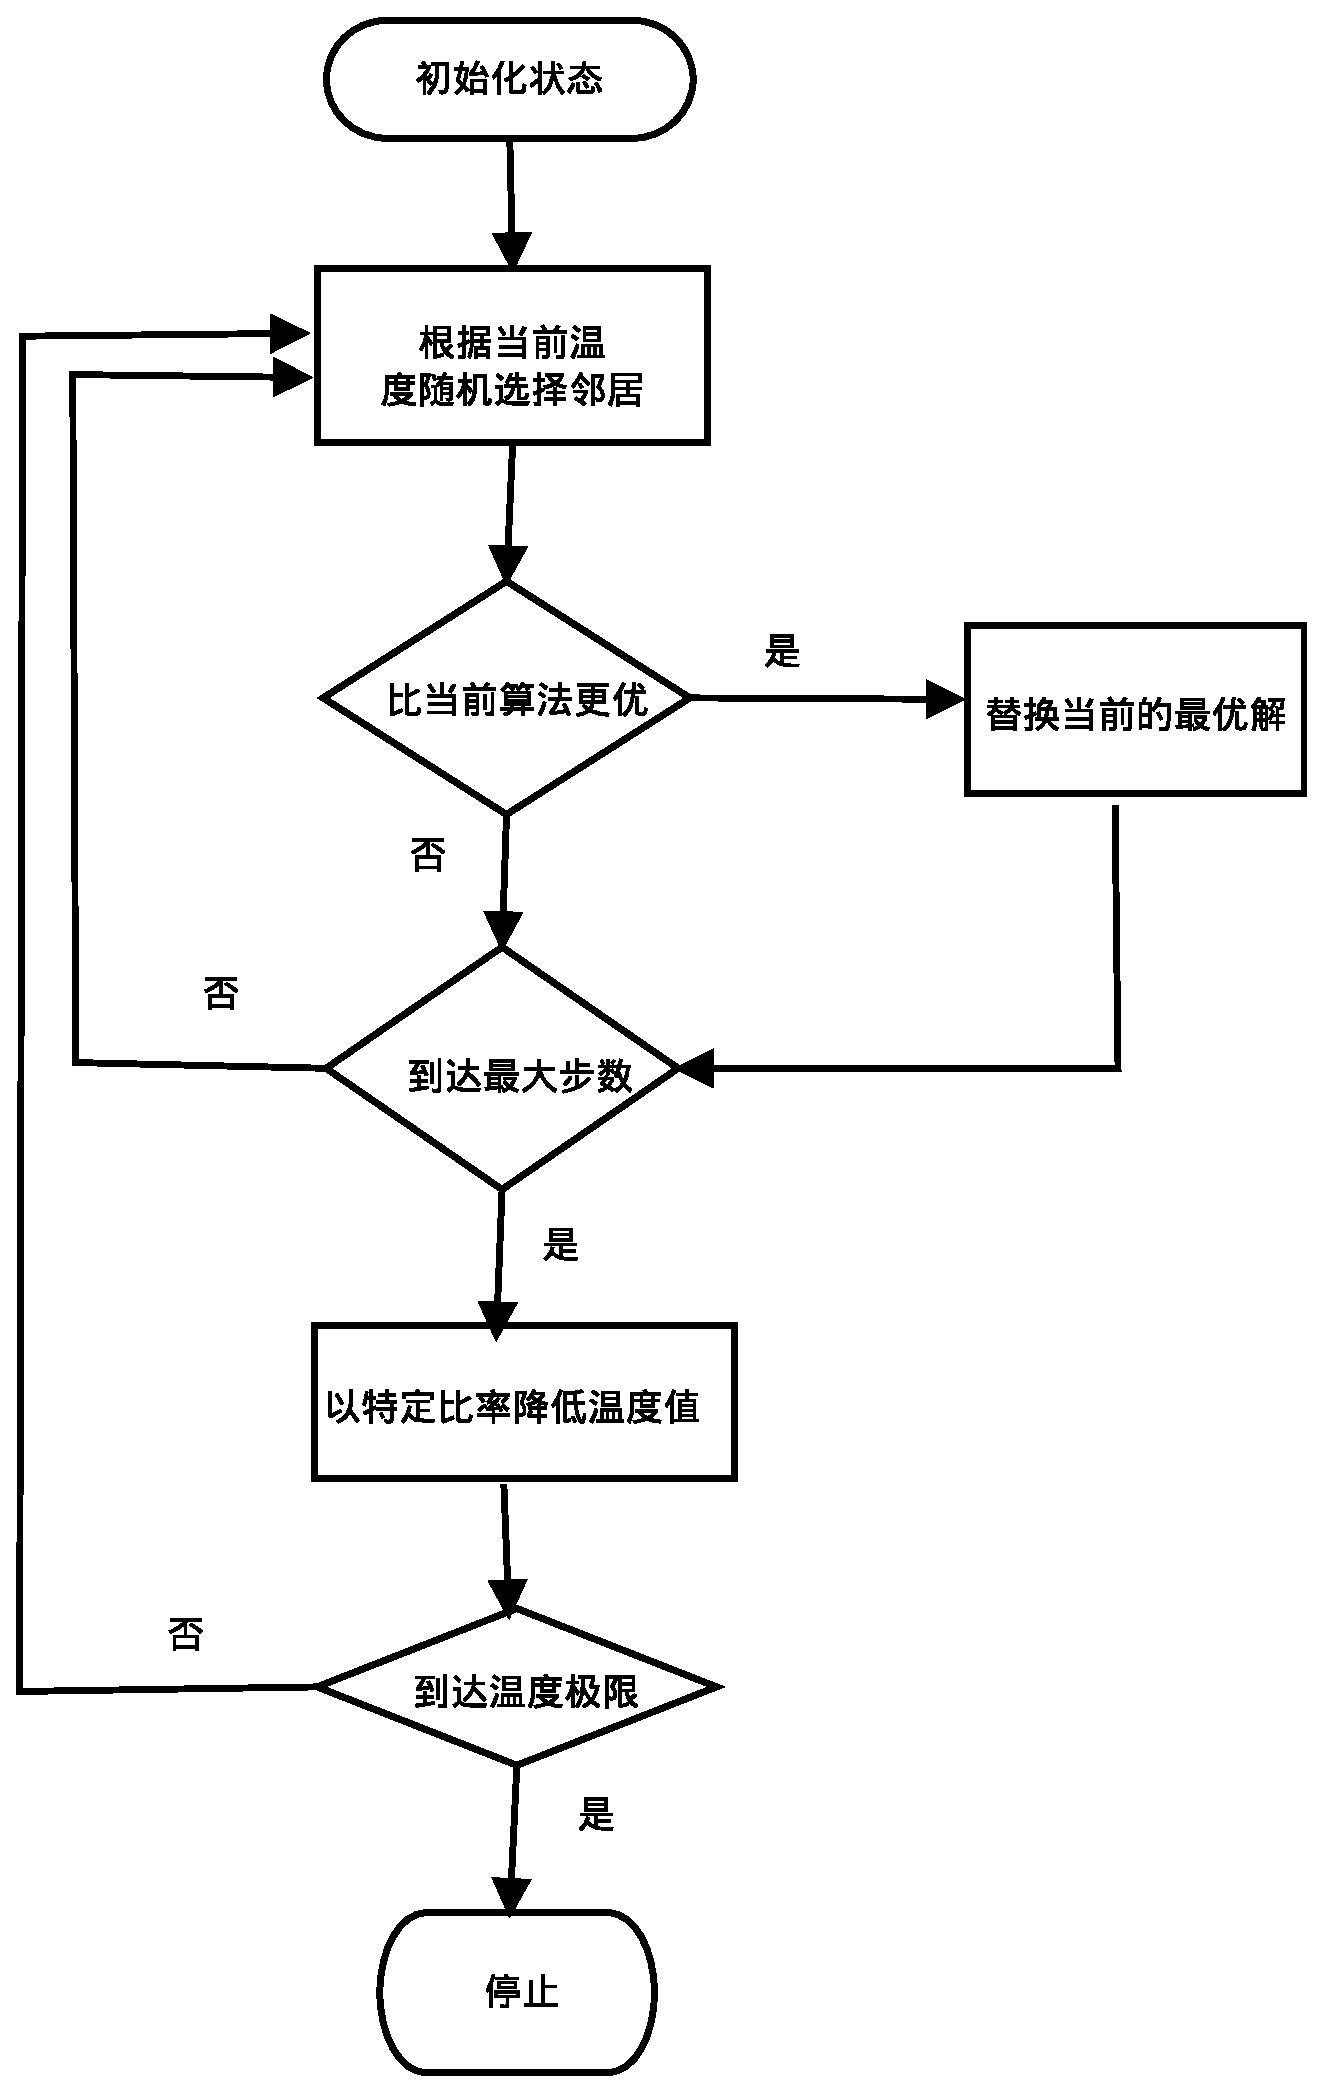
\includegraphics[width=0.6\textwidth]{simulatedannealing}
    \caption{模拟退火算法流程图}\label{fig:simulatedannealing}
    \vspace{\baselineskip}
    \end{figure}

    

\section{并行计算程序性能分析}
    对于给定并行问题需求和特定解决方案,可以构造出不同的算法.如何衡量并行计算的性能成为需要考虑的问题,
加速比做为衡量并行计算性能的重要指标之一,可以衡量并行计算的性能.加速比的公式,
    \[  S[N] = \frac{T_1}{T_N}  \]
其中N是指参与并行计算的CPU数量;$T_1$表示程序在单cpu上运行所需要的时间,$T_N$表示程序在N个CPU上运行所需要的时间
,S(N)则为加速比
    
    通常情况下,程序并不是所有部分都是可以被并行的,会存在着串行部分和可被并行的部分,同时,由于进程见间通讯造成的时间损失,
所以通常加速比无法等于计算机结点的数目,只能接近于计算机节点的数目.S(N)越大,说明并行计算的性能越好,处理效率越高,

    但是S(N)与计算机的数目也有直接的关系,为了更好地衡量并行计算的性能,也可采用算法的并行效率指标,
一般地,$T_N = \frac{T_1}{N}$,所以有$E_N <= 1 $ ,$E_N$越接近于1,说明并行效果越好,

    并行算法的成本主要为时间成本,等于并行机各处理器上运行时间的总和,计算公式可表达为
    
    \[ TimeCost=PxT_p  \]

    评价并行算法的优劣,除了以上3个主要指标意外,还有算法时间复杂度和空间复杂度等.通常情况下,
时间复杂度与算法优劣有关,空间复杂度与算法规模有关.
